% Options for packages loaded elsewhere
\PassOptionsToPackage{unicode}{hyperref}
\PassOptionsToPackage{hyphens}{url}
%
\documentclass[
  english,
]{article}
\usepackage{amsmath,amssymb}
\usepackage{lmodern}
\usepackage{ifxetex,ifluatex}
\ifnum 0\ifxetex 1\fi\ifluatex 1\fi=0 % if pdftex
  \usepackage[T1]{fontenc}
  \usepackage[utf8]{inputenc}
  \usepackage{textcomp} % provide euro and other symbols
\else % if luatex or xetex
  \usepackage{unicode-math}
  \defaultfontfeatures{Scale=MatchLowercase}
  \defaultfontfeatures[\rmfamily]{Ligatures=TeX,Scale=1}
\fi
% Use upquote if available, for straight quotes in verbatim environments
\IfFileExists{upquote.sty}{\usepackage{upquote}}{}
\IfFileExists{microtype.sty}{% use microtype if available
  \usepackage[]{microtype}
  \UseMicrotypeSet[protrusion]{basicmath} % disable protrusion for tt fonts
}{}
\makeatletter
\@ifundefined{KOMAClassName}{% if non-KOMA class
  \IfFileExists{parskip.sty}{%
    \usepackage{parskip}
  }{% else
    \setlength{\parindent}{0pt}
    \setlength{\parskip}{6pt plus 2pt minus 1pt}}
}{% if KOMA class
  \KOMAoptions{parskip=half}}
\makeatother
\usepackage{xcolor}
\IfFileExists{xurl.sty}{\usepackage{xurl}}{} % add URL line breaks if available
\IfFileExists{bookmark.sty}{\usepackage{bookmark}}{\usepackage{hyperref}}
\hypersetup{
  pdftitle={Guidelines for Studies in the Department of Ecological Dynamics of the IZW},
  pdflang={en},
  hidelinks,
  pdfcreator={LaTeX via pandoc}}
\urlstyle{same} % disable monospaced font for URLs
\usepackage[margin=1in]{geometry}
\usepackage{graphicx}
\makeatletter
\def\maxwidth{\ifdim\Gin@nat@width>\linewidth\linewidth\else\Gin@nat@width\fi}
\def\maxheight{\ifdim\Gin@nat@height>\textheight\textheight\else\Gin@nat@height\fi}
\makeatother
% Scale images if necessary, so that they will not overflow the page
% margins by default, and it is still possible to overwrite the defaults
% using explicit options in \includegraphics[width, height, ...]{}
\setkeys{Gin}{width=\maxwidth,height=\maxheight,keepaspectratio}
% Set default figure placement to htbp
\makeatletter
\def\fps@figure{htbp}
\makeatother
\setlength{\emergencystretch}{3em} % prevent overfull lines
\providecommand{\tightlist}{%
  \setlength{\itemsep}{0pt}\setlength{\parskip}{0pt}}
\setcounter{secnumdepth}{-\maxdimen} % remove section numbering
\ifxetex
  % Load polyglossia as late as possible: uses bidi with RTL langages (e.g. Hebrew, Arabic)
  \usepackage{polyglossia}
  \setmainlanguage[]{english}
\else
  \usepackage[main=english]{babel}
% get rid of language-specific shorthands (see #6817):
\let\LanguageShortHands\languageshorthands
\def\languageshorthands#1{}
\fi
\ifluatex
  \usepackage{selnolig}  % disable illegal ligatures
\fi

\title{Guidelines for Studies in the Department of Ecological Dynamics
of the IZW}
\author{}
\date{\vspace{-2.5em}Last Update: July 15, 2021}

\begin{document}
\maketitle

\begin{figure}

\includegraphics[width=1\linewidth]{./src/d6_white} \end{figure}

\textbf{Welcome to the Department of Ecological Dynamics!}

These guidelines are meant to ease your start in the department and to
secure high quality standards for the analysis of your data.

\newpage

\hypertarget{general-information}{%
\section{General Information}\label{general-information}}

The department is composed of three teams on (1) Individual Dynamics,
(2) Population Dynamics and (3) Biodiversity Dynamics.

Stephanie Kramer-Schadt is the department head and leader of the
Population Dynamics team. Conny Landgraf is the assistant of the
department head; she can assist with administrative duties
(e.g.~contracts, travel sheets, etc.). Moritz Wenzler and Jan Axtner are
responsible for data management, data storage and the working group's R
code collection. As each department member has a specific area of
expertise, we created an expert list (see 1.3) if you need help on
specific topics. PhD students and scientists are obliged to update this
expert list with their own skills and responsibilities as well.

For information on the Department, check
\href{https://www.ecological-dynamics-izw.com}{our webpage}
(\url{https://www.ecological-dynamics-izw.com}) or subscribe to
\href{https://www.twitter.com/EcoDynIZW}{our Twitter account}
(@EcoDynIZW) for news about papers, helpful R-code, courses or
scientific positions.

\hypertarget{teams-of-the-department-of-ecological-dynamics}{%
\subsection{Teams of the Department of Ecological
Dynamics:}\label{teams-of-the-department-of-ecological-dynamics}}

\begin{enumerate}
\def\labelenumi{(\arabic{enumi})}
\tightlist
\item
  \emph{Individual Dynamics} -- PI: Sarah Benhaiem
\item
  \emph{Population Dynamics} -- PI: Stephanie Kramer-Schadt \& Viktoriia
  Radchuk
\item
  \emph{Biodiversity Dynamics} -- PI: Andreas Wilting
\end{enumerate}

\hypertarget{administrative-support}{%
\subsection{Administrative support}\label{administrative-support}}

Conny Landgraf\\
Tel: - 466\\
Email: assist6{[}at{]}izw-berlin.de or landgraf{[}at{]}izw-berlin.de

\hypertarget{data-managers}{%
\subsection{Data Managers}\label{data-managers}}

Dr.~Jan Axtner\\
Tel: - 339\\
Email: axtner{[}at{]}izw-berlin.de

Moritz Wenzler-Meya\\
Tel: - 722\\
Email: wenzler{[}at{]}izw-berlin.de

\hypertarget{in-house-experts-scientists-responsibilities}{%
\subsection{In-house experts / scientists /
responsibilities}\label{in-house-experts-scientists-responsibilities}}

Who does what in the department? Tasks and expertise as well as meeting
dates and protocols can be found here:
\texttt{U:\textbackslash{}GUEST\textbackslash{}Abteilung6\textbackslash{}GeneralInfo}

\hypertarget{conducting-bscmscphd-projects}{%
\section{Conducting BSc/MSc/PhD
Projects}\label{conducting-bscmscphd-projects}}

For PhD students: please read the IZW PhD guidelines
(\texttt{\textbackslash{}\textbackslash{}izw-daten-8\textbackslash{}Alle\textbackslash{}GUEST\textbackslash{}Doktorand(inn)en\textbackslash{}IZW-PhD-rules})
carefully and follow the instructions (e.g.~when you have to give an
introduction talk). For any question about these guidelines, contact the
PhD coordinators (currently: Gábor Czirják
(czirjak{[}at{]}izw-berlin.de) and Sarah Benhaiem
(benhaiem{[}at{]}izw-berlin.de)).

\hypertarget{meetings}{%
\subsection{Meetings}\label{meetings}}

\begin{itemize}
\tightlist
\item
  Regular meetings with your supervisor often help to avoid a waste of
  time (see also Appendix C). It is in the responsibility of the student
  to organize and schedule regular meeting with his/ her supervisor or
  the team.
\item
  You can either arrange a fixed date with your supervisor (e.g.~first
  Monday of every month) or schedule them on demand. Please find an
  agreement with your supervisor how to handle this best. Please keep in
  mind that any non-regular meeting should be planned at least two weeks
  ahead.
\item
  Use the IZW outlook calendar to schedule meetings with supervisors and
  colleagues (if you have an IZW Email address). That is: create the
  entry in the calendar and `invite' the others, so that the date/
  location appears in each calendar, with sufficient notice time for the
  automated reminder (i.e.~1 day/ 1 hr).
\item
  Prepare the meetings: Think carefully about your problems/questions
  and write your agenda (what you want to discuss) before the meeting,
  make suggestions for your solution(s) and ask the
  supervisors/collaborators to comment on your solution(s).
\item
  Write the minutes of the meeting and save it in the project folder (we
  give instructions about this project folder below 3.1.). Minimum
  information needed: (1) date of meeting, (2) name of participants, (3)
  questions or problems discussed, (4) main solutions suggested and (5)
  aims or results to prepare for the next meeting. Write down agreements
  of the responsibilities of all collaborators.
\item
  Present your project progress regularly in the department meetings,
  also to get feedback and discuss problems you ran into.
\end{itemize}

\hypertarget{thesis-writing}{%
\subsection{Thesis writing}\label{thesis-writing}}

\begin{itemize}
\tightlist
\item
  Start writing the thesis early enough. Write simple and concise
  sentences based on what is known in the literature. Join a `pub club'
  (i.e.~retreats for writing), e.g.~Team 2 has regular meetings on
  jointly discussing drafts of each other. Please also read the
  instructions (Under construction) for how to write good scientific
  papers.
\item
  Arrange with your supervisor how and in what form you report progress.
  Getting regular feedback for chapters or even just paragraphs might
  keep you from running into dead ends. When asking for revisions plan
  in sufficient time for the reviewers to read and respond (1-3 weeks,
  depending on the amount of text).
\item
  For PhD students: A first complete manuscript draft should be ready
  after \textasciitilde{} 1 year after starting time.
\item
  Send the final version of your manuscript/thesis to all
  supervisors/colleagues at least 4 weeks before the submission date and
  keep in mind that you might have to revise it.
\end{itemize}

\hypertarget{organizing-workflows}{%
\section{Organizing Workflows}\label{organizing-workflows}}

To store data and results, the IZW follows the DFG-guidelines for good
scientific practice. In our department, we often use ``scripting''
(written code of different programming languages) to process and analyze
data, and make results reproducible. Work is structured and organized in
projects and each project will get a project ID from the data
administrators of the department. We consider a project to be a
self-contained topic, e.g.~analyses for a manuscript, thesis chapter,
etc. For each project a separate folder is created and all relevant
scripts, results, the lab-book, documents, literature, minutes of
meetings etc. related to this project are to be kept in that main
folder. For documents (not for scripts!) use your surname, type of
document, project name and in the end the date (\texttt{YYYYMMDD}) as
version numbers for file names
(\texttt{kramer\_manuscript\_lynxibm\_20201231.docx}) and do not use
names like \texttt{doc\_final.docx}, \texttt{doc\_finalfinal.docx},
\texttt{doc\_lastversion.docx} etc. It should contain all information
needed to repeat the study and conduct follow-up studies. Whenever
possible use the standardized project/folder structure shown in section
3.1. Each project or subproject should have a concise but meaningfully
electronic lab-book (see section X.Z) that allows to follow the workflow
and the decisions made in it.

\hypertarget{project-workflow}{%
\subsection{Project workflow}\label{project-workflow}}

Contact the Data Managers (Jan or Moritz) of the respective teams to
organize your project ID, get server access and how to arrange your
workspace best. To setup a project folder, we ask you to follow the
setup:

\begin{itemize}
\tightlist
\item
  The standardized project folder outline! (see Appendix A)
  cf.~\texttt{d6} R package and GitHub)
\item
  Make an outline of the structure separately in your electronic
  lab-book (see 3.3.1), to indicate what to find in each folder and keep
  it updated.
\item
  Please hand over the raw data to the data manager before starting your
  project analysis, to avoid accidental data losses.
\item
  Store the raw data, e.g.~data from field work, in the folder named
  \texttt{data-raw}. Use a folder named \texttt{output} to store data
  created from the raw data (e.g.~after data cleaning or editing). This
  should also be the place where the \texttt{master\ table} is located,
  i.e.~the dataset of all subsequent analyses. If needed you can have a
  temporary subfolder in the ``output'' folder for everyday work and
  analysis trials. Empty the temporary folder regularly. Plots and
  figures should be stored in the \texttt{plots} folder. Scripts should
  be stored in the \texttt{R} folder. Documents like manuscripts,
  proposals, etc. should be stored in the \texttt{docs} folder. Save
  important, computational or labour intensive interim results or final
  results. Use appropriate subfolders such as
  \texttt{interim-results\_\textless{}date\textgreater{}} or
  \texttt{final-results\_\textless{}date\textgreater{}}.
\end{itemize}

\hypertarget{reproducibility}{%
\subsection{Reproducibility}\label{reproducibility}}

To ensure reproducibility and for your own sake always try to script
your work! If possible use R, Python, SQL, etc. for analyses and avoid
manual / mouse commands (e.g.~`clicking' in ArcGIS, QGIS etc.). If you
cannot use scripts, use tools such as the model-builder in ArcGIS or
QGIS and save the drag \& drop model builder scripts.

\hypertarget{documentation}{%
\subsection{Documentation}\label{documentation}}

Project documentation is not a final task, but an ongoing process
starting from day one. DFG guidelines for Safeguarding and Storing of
Primary Data states `Primary data as the basis for publications shall be
securely stored for ten years in a durable form in the institution of
their origin.' Hence, at the end of a research project, you have to hand
over a single well-documented folder per project (usually a paper on the
respective subject, or the BSc thesis) along with all original data. The
project folder should contain all project related documents and data
(e.g.~simulation model codes, simulation results, scripts for
statistical analysis, scripts for tables and figures, manuscripts,
important work documents, applications, permits, reports, etc.) as well
as a the final version of a thesis or paper. Unfinished work (data from
conducted experiments that were not analyzed or published) should
contain the above documents as far as possible, including a very
detailed method description. For the ease of documentation effort please
follow the section (3.3.1).

\hypertarget{electronic-lab-book}{%
\subsubsection{Electronic lab-book}\label{electronic-lab-book}}

At the start of each new project, create an electronic lab-book to
document your workflow and decisions therein. It is of major importance
that you keep this lab-book updated. For the ease of use we recommend
simple .doc files (MS Word, Libre Office etc.) to keep record of our
work. Write down important thoughts, things you have tried, also failed
experiments. Try to use clear and comprehensible notes. Although this
generates some additional effort you will realize soon that it will help
you and others to track your work and make it reproducible. We highly
recommend to use GitHub as version control of your project. You have to
connect your GitHub account to the EcoDynIZW organization on
\href{https://github.com/EcoDynIZW}{GitHub}
(\url{https://github.com/EcoDynIZW}) to share code with colleagues.
Please create repositories on the EcoDynIZW account and not on your
private account! It is mandatory to hand over the electronic lab-book to
the institute as part of the `Safeguarding and Storing of Primary Data'
regulation of the German Research Council DFG after finishing your
project. To document scripting we recommend to use R Markdown
(\texttt{.rmd}) files if possible. Between your code chunks you should
annotate the script with everything that is necessary to understand and
follow the code. Additionally, if you push new code to GitHub for
version control, you have to comment on your committed code as well. It
may be necessary to have an additional word document.

\hypertarget{scripting}{%
\section{Scripting}\label{scripting}}

\hypertarget{general-recommendations}{%
\subsection{General recommendations}\label{general-recommendations}}

\begin{itemize}
\tightlist
\item
  Write the author, name and date in a header (you can use the d6
  package templates for this as well).
\item
  Keep code in scripts as concise as possible.
\item
  Use in-line comments to explain your code that others can follow your
  code.
\item
  If possible, use dynamic paths (i.e.~see R-package
  \href{https://here.r-lib.org/}{\texttt{here}}
  (\url{https://here.r-lib.org/})).
\item
  Always set variables/ parameters at the top of your script; do not set
  values somewhere inside the code as this is error prone, because these
  values tend to be forgotten to get changed when updating a script. The
  same applies to loading packages. Please also make sure to only load
  packages that are really needed and remove those that you are not
  using for the final analysis.
\item
  Save the output of a script as .rds file to smoothly load it in the
  next script. Additionally, save the output in a file format usable
  beyond R, e.g.~use .csv or .txt if you want to save tabular data or
  GeoTiff if you want to save a raster map.
\item
  Use separate scripts to create figures of publishable quality (700
  dpi) from the results. Use a vector graphics format like pdf.
\item
  For simulation studies: Include all scripts, e.g.~additional model
  code, batch files with simulated parameters, simulated landscapes and
  simulation results, and files used for the analyses.
\end{itemize}

\hypertarget{r}{%
\subsection{R}\label{r}}

\begin{itemize}
\tightlist
\item
  Stick to the \href{https://style.tidyverse.org/index.html}{Rstudio
  style guide} (\url{https://style.tidyverse.org/index.html}) to ensure
  readability of code.
\item
  We recommend using R-Studio projects and R Markdown documents when
  scripting in R. If you use another ``integrated development
  environment'' (IDE) make sure you can provide versioned plain R
  scripts using a relative path to the used data files.
\item
  Implement version control by using GitHub. If you install packages or
  use scripts and code chunks from GitHub provided by others, be aware
  to acknowledge the code developer prior to publication of scripts.
\item
  Do not save the R history or the R environment. Always start a fresh
  and an empty R session to avoid artifacts by using objects of
  functions that were not defined in your script. More details here:
  \url{https://www.tidyverse.org/blog/2017/12/workflow-vs-script/}.
\item
  If possible use log files to document messages and errors.
\end{itemize}

\hypertarget{python}{%
\subsection{Python}\label{python}}

In general we recommend using Jupyter notebooks. {[}under
construction{]}

\hypertarget{netlogo}{%
\subsection{Netlogo}\label{netlogo}}

{[}under construction{]}

\hypertarget{qgis}{%
\subsection{QGIS}\label{qgis}}

In general we recommend doing GIS analyses in R. If you have to use QGIS
use Python as scripting language. However, the RQGIS package provides a
great opportunity to script complete workflows in QGIS by using R.
Moreover, you can include R scripts in the QGIS toolbox.

{[}under construction{]}

\hypertarget{spatial-data}{%
\section{Spatial Data}\label{spatial-data}}

If you are working with spatial data please have the following in mind:

\begin{itemize}
\tightlist
\item
  Always check the projection (cartographic reference system (CRS)) of
  your data. Depending on what you want to do it could be necessary to
  change the CRS system, i.e.~from an angular unit (like GPS data) to a
  projected unit in meters. BUT sometimes you cannot easily change it or
  it will drastically change your data.
\item
  If you want to save you spatial data, please save it as Geopackage
  (\texttt{.gpkg}) or raster data GeoTiff (\texttt{.tif}). Please give a
  clear name, document the filename in your lab book and add the EPSG
  code of your CRS to the file name. Always use \texttt{utf-8} as file
  encoding.
\item
  If you are not sure how to handle your spatial data please contact
  Moritz Wenzler, the GIS manager, for help.
\end{itemize}

For detailed information about Spatial data go to Appendix B).

\hypertarget{backup}{%
\section{Backup}\label{backup}}

\textbf{Important:} backup your work! Make copies of raw data/files and
scripts and save it in another location if you work on private
computers. PhD students should work on the M-drive or the U-drive, never
directly on the C-drive of the computer.

\hypertarget{manuscript-submissionsrevisions}{%
\section{Manuscript
Submissions/Revisions}\label{manuscript-submissionsrevisions}}

When you are submitting a manuscript create a copy of the related
subproject folder and add a suffix
\texttt{submission\_1\_\textless{}JournalAbbreviation\textgreater{}}.
This copy shall be stored and never changed (we recommend to zip this
folder)! When conducting a revisions or resubmission, copy the folder to
\texttt{submission\_2\_\textless{}JournalAbbreviation\textgreater{}} and
revise the paper.

Please find additional information on `how to write a scientific paper',
how to avoid statistical pitfalls or how to organize workflows here:
\texttt{U:\textbackslash{}GUEST\textbackslash{}Abteilung6\textbackslash{}LabGuidlines\textbackslash{}D6\_Lab\_Guidelines\_SupplementsToRead},
or on request.

\newpage

\begin{center}\rule{0.5\linewidth}{0.5pt}\end{center}

\textbf{I have read the above guidelines (and Appendices!) and will
follow them.}

Date: \_\_ . \_\_ . \_\_\_\_

Name:
\_\_\_\_\_\_\_\_\_\_\_\_\_\_\_\_\_\_\_\_\_\_\_\_\_\_\_\_\_\_\_\_\_\_\_

Admin:
\_\_\_\_\_\_\_\_\_\_\_\_\_\_\_\_\_\_\_\_\_\_\_\_\_\_\_\_\_\_\_\_\_\_

\begin{center}\rule{0.5\linewidth}{0.5pt}\end{center}

\newpage

\hypertarget{appendix-a-folder-structure-for-project-folders}{%
\section{Appendix A) Folder Structure for Project
Folders}\label{appendix-a-folder-structure-for-project-folders}}

A new project can be started by installing the
\href{https://github.com/EcoDynIZW/d6}{d6 R-package}
(\url{https://github.com/EcoDynIZW/d6}). Running \texttt{new\_project()}
with a unique and descriptive name for your project (see below) will
create a full scaffolding structure for all your future analysis steps.
If you like, you can also specify a path and the project will be created
there.

Please create repositories on the EcoDynIZW account and not on your
private account!

\hypertarget{root-project-folder}{%
\subsection{Root project folder}\label{root-project-folder}}

Name it like:

\textbf{\emph{species\textbar topic\_country\textbar simu\_method\textbar approach\_surname\_firstletterofgivenname}}

e.g.~\emph{unicornus\_wl\_sdm\_smith\_j} (unicornus project in
wonderland, species distribution model from John Smith) or
\emph{stability\_simu\_rpackage\_smith\_j}

\begin{itemize}
\tightlist
\item
  Everything should be written in small letters.
\item
  Avoid spaces or hyphen in the path to the file.
\item
  Species name should be in latin and please use your surname and the
  first letter of your given name at the end.
\item
  Country should be the international abbreviation.
\end{itemize}

The root project folder should hold:

\begin{itemize}
\tightlist
\item
  \textbf{R\_Project\_file}: your main file for your R project (if used)
  --- do not confuse this with R-scripts!

  \begin{itemize}
  \tightlist
  \item
    We highly recommend to use R, but if it is necessary to use another
    programming language and/or program please use the same structure as
    described in the following:
  \end{itemize}
\item
  \textbf{data-raw}: A folder that contains the complete raw dataset
  (e.g.~telemetry data, experiment results, electrophoresis images,
  vegetation survey plots, species lists, etc.).

  \begin{itemize}
  \tightlist
  \item
    Do not use MS Excel files use .csv or .txt files to store/ save
    data.
  \item
    Metadata belonging to the raw data should be provided in a separate
    file but it should be given the same name with an additional suffix
    as the raw data file, e.g.~\emph{area1\_specieslist.txt} or
    \emph{area1\_specieslist\_metadata.txt}
  \end{itemize}
\item
  \textbf{docs}: A folder that contains anything related with project
  administration e.g.~applications, permits, grants, timeline, research
  proposal, the electronic lab-book.
\item
  \textbf{output}: A folder that contains processed raw data

  \begin{itemize}
  \tightlist
  \item
    Results of data preparation and wrangling
  \item
    Results of spatial data processing and spatial analysis,
    e.g.~rasterizing, extracting, calculating on the basic layer and the
    resulting map used for analyses.
  \item
    Final results from analyses
  \end{itemize}
\item
  \textbf{plots}: A folder that contains all produced images for the
  data exploration, presentations, and publications.
\item
  \textbf{R}: A folder that contains all scripts that are used within
  the project.
\item
  If you need additional subfolders add them. Please use also
  second-level subfolders inside the subfolders to keep a clear and tidy
  structure.
\end{itemize}

\begin{figure}
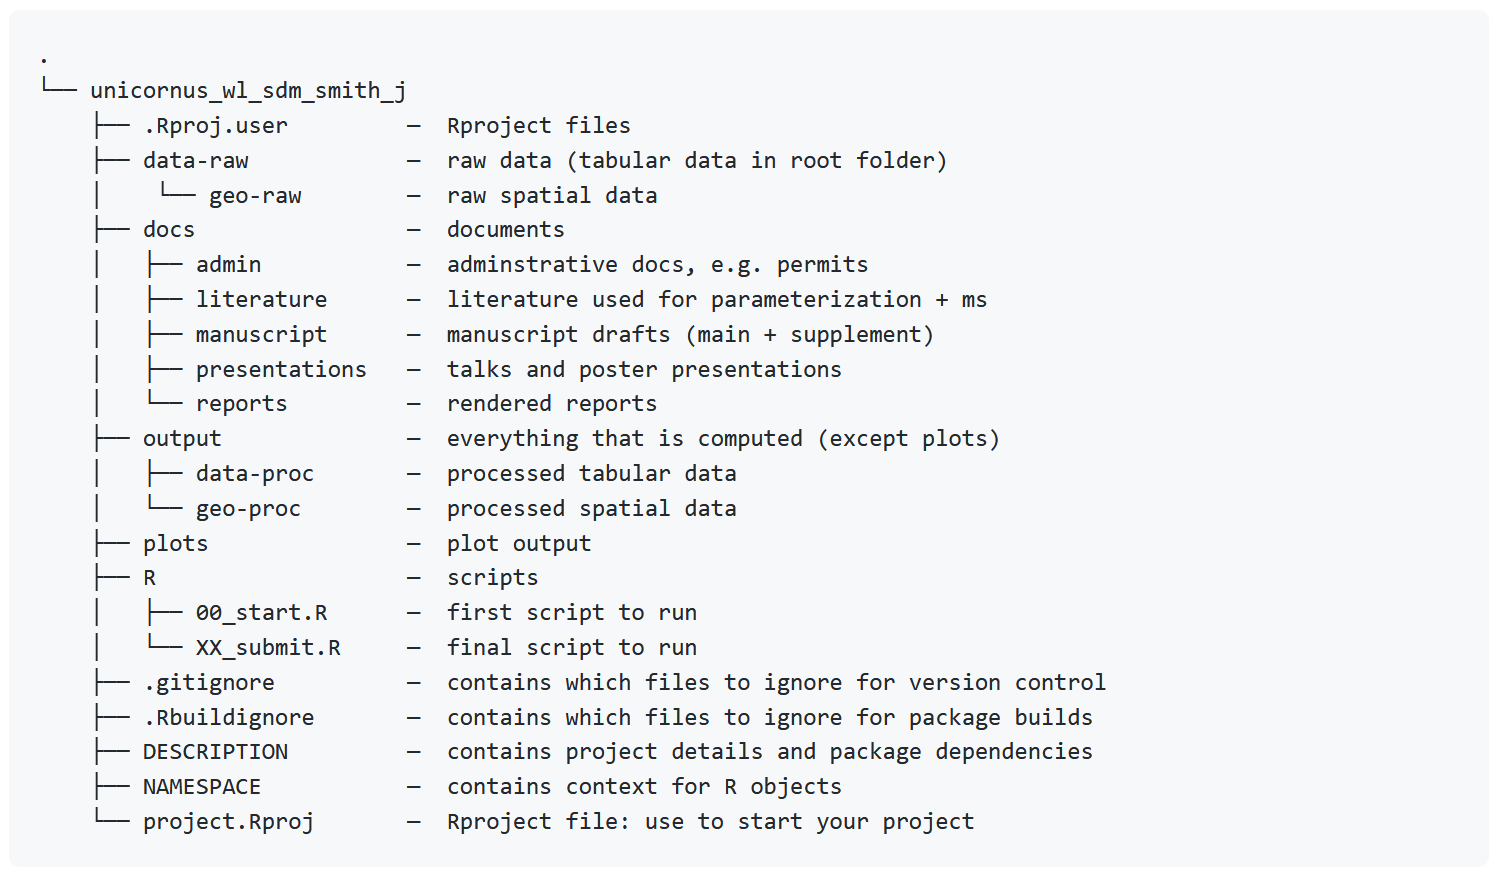
\includegraphics[width=1\linewidth]{./src/folder_structure_d6_projects} \caption{Common project folder strucuture used in the Department of Ecological Dynamics.}\label{fig:unnamed-chunk-2}
\end{figure}

\newpage

\hypertarget{appendix-b-detailed-spatial-data-information}{%
\section{Appendix B) Detailed Spatial Data
Information}\label{appendix-b-detailed-spatial-data-information}}

\begin{itemize}
\tightlist
\item
  When using spatial data give clear names for maps ≤ 13 characters
  without special characters or spaces.
\item
  Write down the cartographic reference system (CRS) at the end of the
  file name, e.g.~\texttt{filename\_4326}.
\item
  Always use \texttt{utf-8} encoding, \textbf{NEVER} use the system
  setting. If you have to use different character encoding settings,
  then name the used encoding in the filename.
\item
  Save the data as geopackage (\texttt{.gpkg}, recommended but cannot be
  used via ArcGis) or shapefile. Geopackages should be the first choice
  as the format is much quicker in every task (loading, saving, changing
  and computing), less limited and OGC-Standard (Open Geospatial
  Consortium). Be aware, that shapefiles have many limitations e.g.~max
  7 characters for column names. Further information is listed in
  Appendix B.
\item
  Crosscheck your scripts and results. If you have calculated
  data/processed maps, make a plot and check for consistency. E.g. there
  should be no data outliers, terrestrial species should not occur in
  the sea etc. If results are valid, mark it as a milestone in your
  project documentation.
\item
  Be aware: if you want to change the coordinate reference system (CRS)
  you have to transform / project the data. Never just specify a new
  one, because this doesn't change the CRS!
\item
  Always include the Coordinate Reference System as EPSG code (e.g.~4326
  for log/lat WGS84 Coordinates) at the end of a file name,
  e.g.~\texttt{my\_env\_variable\_4326.gpkg}.
\item
  Please save all your geo data into geopackage files (\texttt{.gpkg})
  format to save and process your data. In general, if you export data
  from R please save it as an R Studio file (\texttt{.rds}). It will be
  saved without any losses.
\item
  Store all point/line/polygon data as WGS84 (EPSG 4326).
\item
  If you do not understand this paragraph, contact the geodata-manager
  (Moritz Wenzler) before doing anything involving geodata.
\end{itemize}

\newpage

\hypertarget{appendix-c-what-nature-says}{%
\section{Appendix C) What Nature
Says\ldots{}}\label{appendix-c-what-nature-says}}

\emph{Nature \textbf{561}, 277 (2018)}

\textbf{Why you need an agenda for meetings with your principal
investigator}

A list of talking points can help with navigating potentially difficult
topics and sticky negotiations. As PhD students, we often find ourselves
discussing our interactions with our principal investigators (PIs) and
swapping advice for improving our mentoring meetings. We have found
three practices to be consistently helpful: asking our PIs about all
aspects of their job; preparing an agenda for each meeting; and
negotiating new experiments without explicitly saying `no'.

\emph{Read the full text:
\url{https://doi.org/10.1038/d41586-018-06619-3}}

\end{document}
